%% Figure from MATH 556 notes, section 47 (Lecture 21). ADDED (not from lecture).
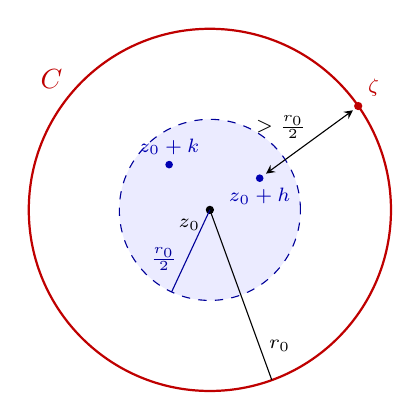
\begin{tikzpicture}[scale=1.15, >=stealth]
    \fill[blue!8] (0,0) circle (1);
    \draw[thick, red!75!black] (0,0) circle (2);
    \draw[dashed, blue!60!black] (0,0) circle (1);
    \fill (0,0) circle (1.3pt) node[below left, font=\scriptsize] {$z_0$};
    \fill[blue!70!black] (0.55,0.35) circle (1.2pt) node[below, font=\scriptsize] {$z_0 + h$};
    \fill[blue!70!black] (-0.45,0.5) circle (1.2pt) node[above, font=\scriptsize] {$z_0 + k$};
    \fill[red!75!black] (1.638,1.147) circle (1.3pt) node[above right, font=\scriptsize] {$\zeta$};
    \draw[<->, thin] (0.62,0.40) -- node[above left, font=\scriptsize, inner sep=1pt] {$> \frac{r_0}{2}$} (1.58,1.10);
    \draw[thin] (0,0) -- node[right, font=\scriptsize, pos=0.8] {$r_0$} (-70:2);
    \draw[thin, blue!60!black] (0,0) -- node[left, font=\scriptsize, pos=0.6] {$\frac{r_0}{2}$} (-115:1);
    \node[red!75!black] at (-1.75,1.45) {$C$};
\end{tikzpicture}
